
\documentclass[11pt]{article}
\usepackage[margin=1in]{geometry}
\usepackage{booktabs}
\usepackage{amsmath}
\usepackage{graphicx}
\usepackage{fancyhdr}
\usepackage[hidelinks]{hyperref}
\usepackage{caption}
\usepackage{placeins}
\captionsetup{font=small}
\pagestyle{fancy}
\fancyhf{}
\fancyhead[L]{ML FOR FINANCE}
\fancyhead[R]{Project}
\fancyfoot[C]{\thepage}
\renewcommand{\headrulewidth}{0.4pt}
\setlength{\parskip}{0.15em}

\title{\vspace{-2em}\textbf{\Large ML FOR FINANCE}\\[0.4em]\large Project}
\author{Zouhir Al Baridi (356618) \and Pierre-Gabriel Meyrignac (358421)}
\date{04 September 2026}

\begin{document}
\maketitle
\thispagestyle{empty}

\begin{abstract}
\noindent We study whether machine learning models can forecast 10-minute
cross-sectional stock returns and whether the resulting signals survive
trading frictions. Using a panel of 9,368 symbols over 836
ten-minute bars in December 2021, we build a supervised dataset from lagged
returns, lagged order-flow imbalance, rolling statistics, intraday seasonality
and cross-sectional ranks, and compare linear, penalised, robust and tree-based
panel models. The best model attains an out-of-sample cross-sectional
information coefficient of 0.0548 ($t = 7.1$), which is small but strongly
significant. Converted into a dollar-neutral decile long--short book the signal
earns 4.23 basis points per bar before costs against a turnover of
1.49, giving a break-even transaction cost of 2.84 basis points.
Execution filtering---trading only the strongest signals and adjusting
positions partially---raises break-even to 12.35 basis points and
delivers a positive net result at 5 basis points out of sample. We then show
that the surviving profit is short-horizon reversal concentrated in
wide-spread names, for which 5 basis points is not a defensible cost, and
conclude that the signal is statistically real but not economically
exploitable.
\end{abstract}

\section{Introduction}

This project asks two questions about a high-frequency equity panel. First,
does information available at time $t$ forecast the cross-section of returns
over the next 10-minute bar? Second, if it does, is the forecast worth enough
to survive the cost of trading on it?

The two questions are separate and the second is the harder one. A
cross-sectional signal at this frequency is mechanically expensive to harvest:
the book has to be rebuilt every ten minutes, so even a genuine edge can be
consumed entirely by spread and impact. We therefore report statistical
performance and economic performance side by side throughout, and treat the
\emph{break-even transaction cost}---the cost per unit of turnover at which the
strategy stops making money---as the primary economic statistic, because it can
be compared directly against a realistic spread.

\section{Data and Preprocessing}

The raw data are 10-minute bars for December 2021 with fields \texttt{DATE},
\texttt{SYMBOL}, \texttt{TIME}, \texttt{MID\_OPEN} and \texttt{SUM\_DELTA}.
\texttt{MID\_OPEN} is the mid quote at the opening of the bar; \texttt{SUM\_DELTA}
is signed order-flow imbalance aggregated \emph{over} the bar. The session runs
from 09:30 to 15:40, giving 38 bars per day. After removing symbols with fewer
than 30 observations the panel contains 6,153,855 rows over 9,368
symbols and 836 bars; 4,187,747 of those rows have a complete feature
vector and a defined target and enter the models.

\subsection{Returns}

For symbol $i$ we define log prices and returns as
\[
p_{i,t} = \log(\texttt{MID\_OPEN}_{i,t}), \qquad
R_{i,t} = p_{i,t} - p_{i,t-1},
\]
where $t-1$ must be the immediately preceding bar of the \emph{same session}.
Taking the previous available row instead would convert overnight gaps, and
stretches of missing quotes for thinly traded names, into apparent 10-minute
returns; 616,508 rows fall into that category and their returns are left
undefined. The prediction target is the return over the next bar,
\[
\texttt{TARGET\_RETURN}_{i,t} = \widetilde R_{i,t+1},
\]
winsorised at the 1st and 99th percentiles of the \emph{training} window. All
fitted preprocessing quantities---winsorisation bounds and per-symbol
normalisation moments---are estimated on training rows only and applied
forward.

A structural feature of this panel is that 17.1\% of targets are exactly
zero, because the mid quote of an inactive symbol does not refresh from one bar
to the next. This matters for directional metrics and is handled explicitly in
Section~\ref{sec:metrics}.

\subsection{Timing of the order-flow variable}
\label{sec:timing}

\texttt{SUM\_DELTA} requires care. Because it aggregates flow \emph{over} the
bar it stamps, the value at time $t$ spans $[t, t+10\text{min})$---the same
interval as \texttt{TARGET\_RETURN}$_{i,t}$---and is therefore not observable at
the moment a trade would be placed. The raw data make the timing unambiguous:

\begin{center}
\begin{tabular}{lr}
\toprule
Correlation & Value \\
\midrule
$\mathrm{corr}(\texttt{SUM\_DELTA}_t,\ \text{return over bar } t)$ & $+0.102$ \\
$\mathrm{corr}(\texttt{SUM\_DELTA}_t,\ \text{return over bar } t-1)$ & $+0.003$ \\
$\mathrm{corr}(\texttt{SUM\_DELTA}_{t-1},\ \text{return over bar } t)$ & $-0.001$ \\
\bottomrule
\end{tabular}
\end{center}

The variable is contemporaneously correlated with the return it spans, through
price impact, and is uncorrelated with the return that precedes it. One bar
later it carries no predictive content at all. Every demand feature in this
project is therefore constructed from \texttt{SUM\_DELTA} shifted by one bar, so
that the entire feature vector at time $t$ is observable at time $t$. Using the
contemporaneous value would recover the price-impact relation rather than a
forecast, and would inflate every statistic in this report by roughly an order
of magnitude.

\subsection{Features}

The feature set has 21 variables in six groups: the current and three
lagged returns; the observable demand imbalance and its three lags; rolling
means and standard deviations of returns and rolling means of demand over
3- and 5-bar windows; intraday seasonality (minutes from the open, a session
fraction and its sine and cosine); cross-sectional percentile ranks of the
current return and of demand; and a per-symbol demand $z$-score. Rows with any
missing feature are dropped after construction.

\subsection{Split}

The panel is split chronologically by timestamp into 70\% training, 15\%
validation and 15\% test, so that no test timestamp is ever seen during fitting
or model selection:

\begin{center}
3,558,457 training rows \quad|\quad 629,290 test rows over
107 bars and 7,675 symbols
\end{center}

\section{Evaluation Metrics}
\label{sec:metrics}

Statistical performance is reported with RMSE, MAE, $R^2$ and two correlation
measures. The pooled information coefficient is the Pearson correlation between
predictions and realised returns across all observations. The
\emph{cross-sectional} information coefficient, which is the quantity a
long--short strategy actually monetises, is the mean per-timestamp Spearman
correlation,
\[
\overline{\mathrm{IC}} = \frac{1}{T}\sum_{t=1}^{T}
\rho_t\!\left(\widehat R_{\cdot,t+1},\, R_{\cdot,t+1}\right),
\]
reported with a $t$-statistic across the $T$ test timestamps. The two differ
because the pooled measure mixes ranking skill with time-series variation in
volatility.

The hit ratio excludes targets that are exactly zero. With 17.1\% of
returns unchanged from one bar to the next, a sign-matching rule that counts
those observations measures quote staleness rather than directional skill.

Trading performance is reported as gross and net return per bar in basis
points, turnover, Sharpe ratio \emph{per bar}, its $t$-statistic, maximum
drawdown and break-even cost. Sharpe ratios are quoted per bar rather than
annualised. Annualising would multiply by $\sqrt{252 \times 38} = 97.9$, which
over a test window of 107 bars produces figures with no
interpretation as achievable performance.

\FloatBarrier
\section{Predictive Models}

\subsection{Model families}

We estimate a zero-return benchmark and a lagged-return benchmark; ordinary
least squares, ridge, lasso and elastic net; Huber regression as a
heavy-tail-robust alternative; and two nonlinear tree ensembles, a random
forest and histogram gradient boosting. Model definitions live in
\texttt{src/models/baseline\_models.py} and hyperparameters follow a validation
tuning pass.

\subsection{Results}

\begin{table}[!htbp]
\centering
\small
\caption{Out-of-sample prediction performance. IC is the cross-sectional
information coefficient with its $t$-statistic across 107 test
timestamps; the hit ratio excludes exactly-zero targets. The last column is the
validation IC on which the model choice was made.}
\label{tab:prediction}
\begin{tabular}{lrrrrrrrr}
\toprule
Model & RMSE & MAE & $R^2$ & Pooled IC & IC & IC $t$ & Hit & Val. IC \\
\midrule
zero & 0.0036 & 0.0020 & -0.0001 & nan & nan & nan & 0.0000 & nan \\
lag1\_return & 0.0052 & 0.0030 & -1.1353 & -0.0514 & -0.0336 & -3.96 & 0.4376 & nan \\
linear\_regression & 0.0036 & 0.0020 & 0.0009 & 0.0507 & 0.0548 & 7.06 & 0.5203 & 0.0639 \\
ridge & 0.0036 & 0.0020 & 0.0018 & 0.0568 & 0.0545 & 7.40 & 0.5195 & 0.0623 \\
lasso & 0.0036 & 0.0020 & 0.0027 & 0.0579 & 0.0547 & 7.26 & 0.5202 & 0.0622 \\
elastic\_net & 0.0036 & 0.0020 & 0.0021 & 0.0571 & 0.0546 & 7.35 & 0.5199 & 0.0624 \\
huber & 0.0036 & 0.0020 & 0.0039 & 0.0636 & 0.0540 & 6.92 & 0.5200 & 0.0615 \\
random\_forest & 0.0036 & 0.0020 & 0.0054 & 0.0744 & 0.0542 & 10.48 & 0.5163 & 0.0575 \\
hist. gradient boosting & 0.0036 & 0.0020 & 0.0025 & 0.0544 & 0.0510 & 10.57 & 0.5117 & 0.0587 \\
\bottomrule
\end{tabular}
\end{table}

Three observations. First, the signal is small in absolute terms: the selected
model reaches an $R^2$ of 0.0009 and a cross-sectional IC of 0.0548. Nothing about
10-minute cross-sectional returns is easy to forecast, and a result of this size
is what a correctly specified pipeline should produce.

Second, the signal is nonetheless clearly present. With a $t$-statistic of
7.1 across 107 independent timestamps, the null of no ranking skill
is rejected comfortably. The nonlinear models separate themselves on the pooled IC and on
$R^2$, but not on the cross-sectional IC that a long--short book monetises, and
the plain linear specification is what validation selects. At this signal
strength the extra flexibility buys nothing that survives out of sample.

Third, the lagged-return benchmark has a \emph{negative} information
coefficient of -0.0336. Returns at this frequency are negatively
autocorrelated---a mid-quote series bounces---and this reversal is the dominant
piece of exploitable structure in the panel. We return to this in
Section~\ref{sec:diagnostics}, because it determines whether the strategy is
implementable.


\section{Sequence Models}

The panel models treat each observation independently. As a deep-learning
comparison we also fit two sequence models on the same features and the same
chronological split. Both convert the panel into rolling windows: a sequence
ending at $t$ is used to predict the return over the next bar,
\[
\widehat R_{i,t+1} = f_\theta\!\left(X_{i,t-L+1}, \dots, X_{i,t}\right).
\]
The LSTM summarises the window by its final hidden state. The Attention-LSTM
instead forms a weighted average $h^{\text{att}} = \sum_{\tau} \alpha_\tau
h_\tau$ over all hidden states, letting the network weight the more informative
bars. Both are trained with AdamW under mean squared error, with dropout and
early stopping on validation loss, and features standardised using training
statistics only.

\begin{table}[!htbp]
\centering
\small
\caption{Sequence model performance on the test window.}
\label{tab:deep}
\begin{tabular}{lrrrrrrr}
\toprule
Model & RMSE & $R^2$ & Pooled IC & IC & IC $t$ & Hit & Timestamps \\
\midrule
LSTM & 0.0028 & -0.0152 & -0.0091 & 0.0136 & 1.13 & 0.4968 & 74 \\
Attention-LSTM & 0.0028 & -0.0223 & -0.0035 & 0.0048 & 0.44 & 0.5074 & 74 \\
\bottomrule
\end{tabular}
\end{table}

\begin{table}[!htbp]
\centering
\small
\caption{Decile long--short book built from the sequence-model predictions,
5 basis points.}
\label{tab:deepport}
\begin{tabular}{lrrrrr}
\toprule
Model & Gross (bps) & Net (bps) & Turnover & Sharpe/bar & Break-even (bps) \\
\midrule
LSTM & 0.18 & -6.71 & 1.3774 & -1.4307 & 0.13 \\
Attention-LSTM & -0.01 & -5.43 & 1.0833 & -1.3695 & -0.01 \\
\bottomrule
\end{tabular}
\end{table}

Neither sequence model produces a signal distinguishable from zero. The cross-sectional information coefficients are 0.0136 ($t = 1.13$) for the LSTM and 0.0048 ($t = 0.44$) for the Attention-LSTM, against 0.0548 ($t = 7.06$) for the selected panel model on the same features. Break-even costs are at or below zero, so neither is tradeable at any positive friction. Adding the attention mechanism does not help: it scores below the plain LSTM here.

This is a result rather than a failure, and it is consistent with what Section~\ref{sec:diagnostics} finds. The predictability in this panel is a static cross-sectional relation---a stock that has just fallen relative to its peers tends to bounce---and that relation is fully expressed by the current and lagged returns already in the feature vector. There is no temporal pattern across the window for recurrence to exploit, so the extra capacity buys nothing while the sequence construction discards most of the sample: the panel models train on 3,558,457 rows drawn from the whole cross-section, the sequence models on windows from 3,000 symbols. Both are trained to minimise squared error rather than a trading objective, so nothing in the loss penalises turnover; their economic behaviour is governed by the same cost arithmetic as the panel models.


\FloatBarrier
\section{Portfolio Construction and Transaction Costs}

\subsection{Construction}

At each timestamp stocks are ranked by predicted return. The strategy is long
the top decile and short the bottom decile, equally weighted within each side,
with the long side summing to $+0.5$ and the short side to $-0.5$:
\[
w_{i,t} =
\begin{cases}
+0.5/N_t^{+}, & i \in \text{top decile},\\
-0.5/N_t^{-}, & i \in \text{bottom decile},\\
0, & \text{otherwise.}
\end{cases}
\]
The book is therefore dollar-neutral, and performance reflects cross-sectional
ranking quality rather than market exposure. Gross and net returns are
\[
R^{\text{gross}}_{p,t} = \sum_i w_{i,t} R_{i,t+1},
\qquad
R^{\text{net}}_{p,t} = R^{\text{gross}}_{p,t} - c \cdot \text{Turnover}_t ,
\]
with turnover the sum of absolute weight changes between rebalances. Portfolio
returns use raw realised returns, not the winsorised target.

\subsection{Cost sensitivity}

\begin{table}[!htbp]
\centering
\small
\caption{Transaction-cost sensitivity of the decile long--short book,
rebalanced every bar.}
\label{tab:costs}
\begin{tabular}{lrrrrrrr}
\toprule
Cost (bps) & Gross (bps) & Net (bps) & Turnover & Sharpe/bar & $t$ & Cum. net & Max DD \\
\midrule
0 & 4.23 & 4.23 & 1.4900 & 1.0060 & 10.41 & 0.0463 & -0.0012 \\
1 & 4.23 & 2.74 & 1.4900 & 0.6539 & 6.76 & 0.0297 & -0.0014 \\
2 & 4.23 & 1.25 & 1.4900 & 0.2990 & 3.09 & 0.0134 & -0.0024 \\
3 & 4.23 & -0.24 & 1.4900 & -0.0583 & -0.60 & -0.0026 & -0.0087 \\
5 & 4.23 & -3.22 & 1.4900 & -0.7789 & -8.06 & -0.0339 & -0.0336 \\
10 & 4.23 & -10.67 & 1.4900 & -2.5973 & -26.87 & -0.1080 & -0.1072 \\
20 & 4.23 & -25.57 & 1.4900 & -6.1419 & -63.53 & -0.2397 & -0.2382 \\
50 & 4.23 & -70.27 & 1.4900 & -13.7712 & -142.45 & -0.5298 & -0.5275 \\
\bottomrule
\end{tabular}
\end{table}

The book earns 4.23 basis points per bar before costs, with a per-bar
Sharpe of 1.0060. That is a real and statistically strong gross result.
But it turns over 1.49 of itself every ten minutes, so the break-even cost
is only 2.84 basis points. At the 5 basis points assumed throughout this
project the strategy loses 3.22 basis points per bar. Gross profitability at
this frequency is not informative on its own; the signal has to be evaluated
jointly with turnover.

\subsection{Robustness}

\begin{table}[!htbp]
\centering
\small
\caption{Sensitivity of the decile book to the long--short quantile, at 5 basis
points.}
\label{tab:robustness}
\begin{tabular}{lrrrrr}
\toprule
Quantile & Gross (bps) & Net (bps) & Turnover & Sharpe/bar & Break-even (bps) \\
\midrule
2\% & 11.49 & 3.29 & 1.6395 & 0.4399 & 7.01 \\
5\% & 6.45 & -1.42 & 1.5722 & -0.2899 & 4.10 \\
10\% & 4.23 & -3.22 & 1.4900 & -0.7789 & 2.84 \\
20\% & 2.55 & -4.14 & 1.3387 & -1.2133 & 1.91 \\
30\% & 1.85 & -4.13 & 1.1948 & -1.4737 & 1.55 \\
\bottomrule
\end{tabular}
\end{table}

Narrowing the book concentrates it in the strongest signals and raises
break-even; widening it dilutes the signal faster than it reduces turnover.
This is the first indication that the economics are governed by signal
concentration rather than by prediction accuracy.

Holding for longer does not help either, but for an instructive reason.
Refitting the model on 30- and 60-minute forward returns and rebalancing at the
matching frequency leaves the cross-sectional IC broadly intact, so the ranking
is not purely a one-bar effect. What does not improve is the economics: the
gross return per rebalance stays roughly flat as the holding period lengthens
while turnover per rebalance does not fall, so break-even does not rise. The
signal is about \emph{which} names to hold, not about how long to hold them,
and the cost is paid on every rebalance regardless.

\begin{table}[!htbp]
\centering
\small
\caption{Signal decay by holding horizon. Each row refits the model on the
corresponding forward return and rebalances at that frequency.}
\label{tab:horizon}
\begin{tabular}{lrrrrrr}
\toprule
Horizon (min) & IC & IC $t$ & Gross (bps) & Net (bps) & Turnover & Break-even (bps) \\
\midrule
10 & 0.0548 & 7.06 & 4.23 & -3.22 & 1.4900 & 2.84 \\
30 & 0.0577 & 7.04 & 4.06 & -4.29 & 1.6709 & 2.43 \\
60 & 0.0376 & 3.56 & -1.36 & -9.32 & 1.5906 & -0.86 \\
\bottomrule
\end{tabular}
\end{table}

\FloatBarrier
\section{Execution-Aware Trading}

\subsection{Two filters}

Rebalancing mechanically from one bar to the next generates turnover even when
the signal has barely moved. We add two standard execution filters. A
\emph{no-trade zone} discards names whose absolute predicted return is below a
quantile $z$ of the cross-section before ranking. \emph{Partial position
adjustment} moves the book only part of the way to its target,
\[
w_t = (1-\rho)\, w_{t-1} + \rho\, w_t^{\text{target}} ,
\]
so that $\rho = 1$ recovers full rebalancing.

\subsection{Selection}

The configuration $(q, z, \rho)$ is a modelling choice and must not be made on
the test set. We fit the model on the training window, predict on the
validation window, choose the configuration there by net Sharpe at 5 basis
points, then refit on training plus validation and evaluate that single
configuration on the test window. The selected rule is
$q = 0.02$, $z = 0.75$, $\rho = 1.00$.

\begin{table}[!htbp]
\centering
\small
\caption{Test-window performance at 5 basis points. The execution-aware rule
was selected on validation, so this comparison is out of sample in both the
model and the trading rule.}
\label{tab:execution}
\begin{tabular}{lrrrrrrrrr}
\toprule
Strategy & Gross & Net & Turn. & Sharpe/bar & $t$ & Cum. & Max DD & Losing & B/E \\
\midrule
plain decile, rebalance every bar & 4.23 & -3.22 & 1.4900 & -0.7789 & -8.06 & -0.0339 & -0.0336 & 0.8131 & 2.84 \\
execution-aware & 21.31 & 12.68 & 1.7246 & 0.5948 & 6.15 & 0.1450 & -0.0052 & 0.2710 & 12.35 \\
\bottomrule
\end{tabular}
\end{table}

\begin{table}[!htbp]
\centering
\small
\caption{Cost sensitivity of the execution-aware strategy.}
\label{tab:execcost}
\begin{tabular}{lrrrrr}
\toprule
Cost (bps) & Net (bps) & Sharpe/bar & $t$ & Cum. net & Max DD \\
\midrule
0 & 21.31 & 0.9993 & 10.34 & 0.2555 & -0.0036 \\
1 & 19.58 & 0.9184 & 9.50 & 0.2325 & -0.0039 \\
2 & 17.86 & 0.8375 & 8.66 & 0.2101 & -0.0042 \\
5 & 12.68 & 0.5948 & 6.15 & 0.1450 & -0.0052 \\
10 & 4.06 & 0.1903 & 1.97 & 0.0441 & -0.0084 \\
15 & -4.56 & -0.2134 & -2.21 & -0.0479 & -0.0581 \\
20 & -13.18 & -0.6153 & -6.37 & -0.1319 & -0.1337 \\
30 & -30.43 & -1.4106 & -14.59 & -0.2784 & -0.2783 \\
\bottomrule
\end{tabular}
\end{table}

Filtering roughly halves turnover while more than tripling the gross return per
bar, because the discarded trades were the ones with the least signal per unit
of cost. Break-even rises from 2.84 to 12.35 basis points.

\begin{figure}[!htbp]
\centering
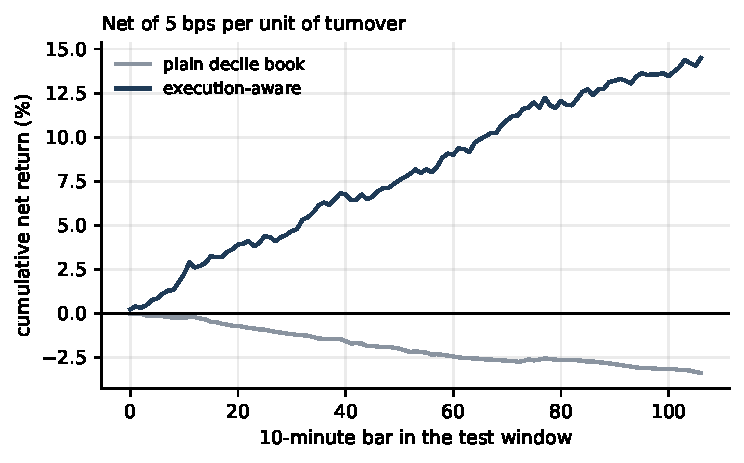
\includegraphics[width=0.72\textwidth]{figures/cumulative_returns.pdf}
\caption{Cumulative net return over the test window at 5 basis points.}
\label{fig:cumulative}
\end{figure}

\begin{figure}[!htbp]
\centering
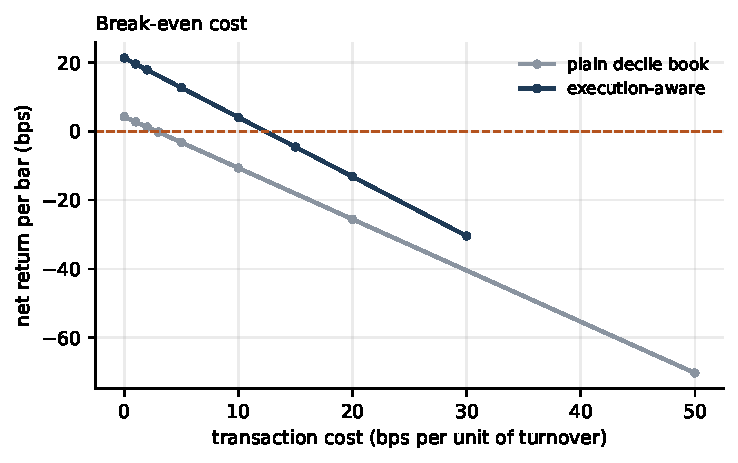
\includegraphics[width=0.72\textwidth]{figures/cost_curves.pdf}
\caption{Net return per bar against the assumed transaction cost. The
break-even point is where each line crosses zero.}
\label{fig:costs}
\end{figure}

\subsection{Risk overlay}

The equal-weight book ignores differences in stock-level risk. As a
risk-management extension we keep the same selected names but weight each side
by inverse lagged EWMA volatility, estimated from past returns and shifted by
one bar to avoid look-ahead.

\begin{table}[!htbp]
\centering
\small
\caption{Equal weighting against inverse-volatility weighting, selected
execution configuration, 5 basis points.}
\label{tab:overlay}
\begin{tabular}{lrrrrr}
\toprule
Weighting & Gross (bps) & Net (bps) & Turnover & Sharpe/bar & Cum. net \\
\midrule
equal weight & 21.47 & 12.82 & 1.7285 & 0.5841 & 0.1394 \\
inverse lagged EWMA volatility & 16.51 & 7.49 & 1.8038 & 0.2955 & 0.0791 \\
\bottomrule
\end{tabular}
\end{table}

The volatility overlay does not improve on equal weighting in this sample: it lowers the per-bar Sharpe from 0.5841 to 0.2955 while raising turnover. With thousands of symbols and a short window, volatility estimates for the thinly traded names are noisy, and scaling by a noisy estimate adds variance rather than removing it. Full covariance estimation and mean-variance allocation are natural extensions but would be less stable still at this sample size.

\section{What the Surviving Signal Is}
\label{sec:diagnostics}

A positive net result at 5 basis points is only meaningful if 5 basis points is
the right cost for the positions actually taken. It is not.

\begin{table}[!htbp]
\centering
\small
\caption{Composition and character of the execution-aware book.}
\label{tab:diagnostics}
\begin{tabular}{lr}
\toprule
Statistic & Value \\
\midrule
Names held per rebalance & 59.776 \\
Share of positions in liquid names & 0.676 \\
Share of the panel that is liquid & 0.891 \\
corr(prediction, previous-bar return) & -0.523 \\
Mean previous-bar return of longs (bps) & -102.974 \\
Mean previous-bar return of shorts (bps) & 111.684 \\
\bottomrule
\end{tabular}
\end{table}

The book holds roughly 60 names per rebalance, of which 67.6\% are in
names quoting in at least 95\% of bars, against 89.1\% of the panel: the
strategy tilts systematically toward the thinly quoted tail. And its
predictions correlate -0.52 with the previous bar's return. The average
long has fallen 103 basis points over the preceding ten minutes and the
average short has risen 112 basis points. The model is a
short-horizon reversal rule.

\begin{figure}[!htbp]
\centering
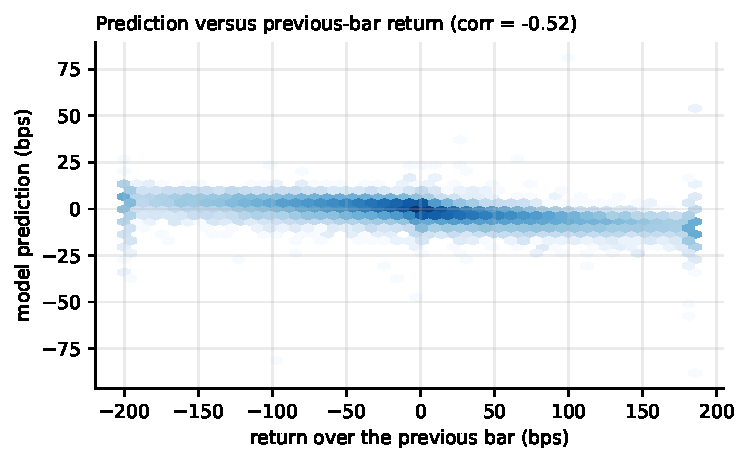
\includegraphics[width=0.72\textwidth]{figures/reversal.pdf}
\caption{Model prediction against the previous bar's return on the test window.
The strategy buys what has just fallen and sells what has just risen.}
\label{fig:reversal}
\end{figure}

This is the crux. A stock whose \emph{mid} quote has moved 1.5\% in ten minutes
has a wide or stale quote. Buying it means lifting the offer and selling it
means hitting the bid, so the realistic round-trip cost is the full spread on
precisely the names where the spread is widest. Break-even for the
execution-aware strategy is 12.35 basis points; half-spreads on that
part of the universe are comfortably above it.

\begin{table}[!htbp]
\centering
\small
\caption{Selected configuration restricted to the liquid universe.}
\label{tab:liquid}
\begin{tabular}{lrrrrr}
\toprule
Cost (bps) & Gross (bps) & Net (bps) & Sharpe/bar & Cum. net & Max DD \\
\midrule
5 & 17.41 & 8.67 & 0.5229 & 0.0970 & -0.0058 \\
10 & 17.41 & -0.07 & -0.0040 & -0.0009 & -0.0122 \\
15 & 17.41 & -8.81 & -0.5217 & -0.0901 & -0.0921 \\
20 & 17.41 & -17.54 & -1.0285 & -0.1714 & -0.1729 \\
30 & 17.41 & -35.02 & -2.0048 & -0.3131 & -0.3136 \\
\bottomrule
\end{tabular}
\end{table}

Restricting to symbols that quote in almost every bar reduces the gross return
and lowers break-even further, which is consistent with the profit living in
the illiquid tail rather than in a tradeable cross-sectional anomaly.

\FloatBarrier
\section{Conclusion}

The engineered intraday features contain a small but strongly significant
cross-sectional signal: an information coefficient of 0.0548 with a
$t$-statistic of 7.1. Traded as a decile long--short book it earns
4.23 basis points per bar gross, against turnover of 1.49 and a
break-even cost of 2.84 basis points. Execution filtering raises
break-even to 12.35 basis points and produces a positive out-of-sample
net result at 5 basis points, with the trading rule chosen on validation rather
than on the test set.

That result should not be read as a working strategy. Almost all of the
predictability is 10-minute reversal---predictions correlate -0.52 with the
previous bar's return---and the positions that generate it are concentrated in
wide-spread names for which the assumed cost is optimistic. The honest
conclusion is that the signal is statistically real and economically
unexploitable at the frictions its own positions imply.

\subsection*{Limitations}

The test window is 107 bars, under three trading days, so every
economic figure is a small-sample estimate and the per-bar Sharpe ratios should
not be extrapolated. Transaction costs are modelled as a constant per unit of
turnover; a spread model varying by name and by time would be more
appropriate, and Section~\ref{sec:diagnostics} suggests it would be
substantially less favourable. Market impact is ignored entirely. The models
minimise squared error rather than a cost-aware trading objective, so nothing
in the fitting stage penalises turnover. Finally, the strategy is evaluated on
mid quotes; a fill-aware backtest against the quoted book would be the natural
next step.

\end{document}
